The large-scale test site Merkers benefits from the unique mining situation in the bedded salt mass of the Werra salt formation (z1, Zechstein sequence) where two potash seams were mined in a room-and-pillar system at 275 m (1st floor, potash seam ''Hessen'', z1KH) and 360 m (2nd floor, potash seam ''Thüringen'', z1KTh) depth, respectively. Fig. \ref{fig:springenlab} shows the preparation of an experiment on the 2nd seam. The evaporite rocks of the Zechstein formation were laid down during the Permian period around 250 million years ago. The intact mineral deposit was locally disturbed between 14 and 25 million years ago by tertiary volcanism, leading to the mutation of some potash salts to sylvinite, and the creation of pockets of CO$_2$ under high pressure.

\begin{figure}
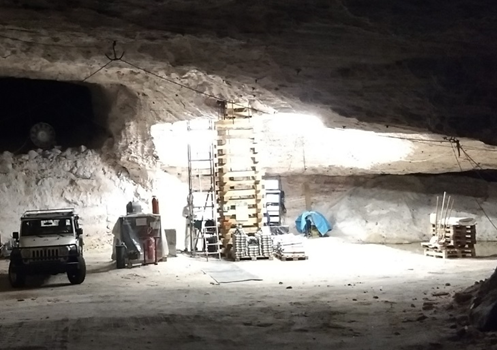
\includegraphics[width=0.7\textwidth]{figures/springen2ndseam.png}
\caption{Preparation of experiments on the second seam.}
\label{fig:springenlab}
\end{figure}

The pressurized tests are conducted between the two potash seams in the very homogeneous Middle Werra rocksalt (z1Na). It consists mostly of very pure halite layers intersected by thin anhydrite lines or bands of rocksalt with finely distributed anhydrite accessories indicating the sedimentary bedding. 

Because the test results depend mainly on the acting stress field, i.e. the minimal stress distribution in the rock mass around the test area, it has been measured and  characterized by hydro-frac measurements, and is thus well-known. The minimal stresses in the contour increase with progressive distances from the underground openings until reaching a constant value in a depth of around 15 m. The measured value of an undisturbed stress state of around 8 MPa corresponds fairly well to calculated lithostatic stresses of 7.8 to 8.8 MPa. 

The main facility is a large borehole of nearly vertical 60 m height and 1.3 m diameter. It was drilled upwards from the second floor, ending about 20 m beneath the first floor. For access to the later sealed volume an 85 mm pilot hole has been drilled from the upper floor. The borehole was closed by a 20 m high MgO-concrete plug. 

For monitoring of micro-seismic events, e.g. due to creation of an excavated damage zone around underground openings or fluid flow driven damage, a highly sensitive AE-network was installed in observation boreholes, which were drilled parallel to the main borehole. This network has constantly been updated and extended over the past years. Signals of magnitude M $<$ -4 can be detected in a frequency range from 1 kHz to 200 kHz. This corresponds to intergranular microcracking on grain boundaries on a millimeter- to centimeter-scale. 
